\documentclass[a4paper,11pt]{article}
\usepackage{amsmath,amsthm,amsfonts,amssymb,amscd,amstext,vmargin,graphics,graphicx,tabularx,multicol} 
\usepackage[francais]{babel}
\usepackage[utf8]{inputenc}  
\usepackage[T1]{fontenc} 
\usepackage{pstricks-add,tikz,tkz-tab,variations}
\usepackage[autolanguage,np]{numprint} 

\setmarginsrb{1.5cm}{0.5cm}{1cm}{0.5cm}{0cm}{0cm}{0cm}{0cm} %Gauche, haut, droite, haut
\newcounter{numexo}
\newcommand{\exo}[1]{\stepcounter{numexo}\noindent{\bf Exercice~\thenumexo} : \marginpar{\hfill /#1}}
\reversemarginpar


\newcounter{enumtabi}
\newcounter{enumtaba}
\newcommand{\q}{\stepcounter{enumtabi} \theenumtabi.  }
\newcommand{\qa}{\stepcounter{enumtaba} (\alph{enumtaba}) }
\newcommand{\initq}{\setcounter{enumtabi}{0}}
\newcommand{\initqa}{\setcounter{enumtaba}{0}}

\newcommand{\be}{\begin{enumerate}}
\newcommand{\ee}{\end{enumerate}}
\newcommand{\bi}{\begin{itemize}}
\newcommand{\ei}{\end{itemize}}
\newcommand{\bp}{\begin{pspicture*}}
\newcommand{\ep}{\end{pspicture*}}
\newcommand{\bt}{\begin{tabular}}
\newcommand{\et}{\end{tabular}}
\renewcommand{\tabularxcolumn}[1]{>{\centering}m{#1}} %(colonne m{} centrée, au lieu de p par défault) 
\newcommand{\tnl}{\tabularnewline}

\newcommand{\bmul}[1]{\begin{multicols}{#1}}
\newcommand{\emul}{\end{multicols}}

\newcommand{\trait}{\noindent \rule{\linewidth}{0.2mm}}
\newcommand{\hs}[1]{\hspace{#1}}
\newcommand{\vs}[1]{\vspace{#1}}

\newcommand{\N}{\mathbb{N}}
\newcommand{\Z}{\mathbb{Z}}
\newcommand{\R}{\mathbb{R}}
\newcommand{\C}{\mathbb{C}}
\newcommand{\Dcal}{\mathcal{D}}
\newcommand{\Ccal}{\mathcal{C}}
\newcommand{\mc}{\mathcal}

\newcommand{\vect}[1]{\overrightarrow{#1}}
\newcommand{\ds}{\displaystyle}
\newcommand{\eq}{\quad \Leftrightarrow \quad}
\newcommand{\vecti}{\vec{\imath}}
\newcommand{\vectj}{\vec{\jmath}}
\newcommand{\Oij}{(O;\vec{\imath}, \vec{\jmath})}
\newcommand{\OIJ}{(O;I,J)}


\newcommand{\reponse}[1][1]{%
\multido{}{#1}{\makebox[\linewidth]{\rule[0pt]{0pt}{20pt}\dotfill}
}}

\newcommand{\titre}[5] 
% #1: titre #2: haut gauche #3: bas gauche #4: haut droite #5: bas droite
{
\noindent #2 \hfill #4 \\
#3 \hfill #5

\vspace{-1.6cm}

\begin{center}\rule{6cm}{0.5mm}\end{center}
\vspace{0.2cm}
\begin{center}{\large{\textbf{#1}}}\end{center}
\begin{center}\rule{6cm}{0.5mm}\end{center}
}



\begin{document}
\pagestyle{empty}
\titre{Interrogation sur les statistiques (1)}{Nom :}{Prénom :}{Classe}{Date}

\begin{flushleft}
\begin{tabular}{|m{9.5cm}|m{1.25cm}|m{1.25cm}|m{1.25cm}|m{1.25cm}|m{1.25cm}|}
\hline 
\textbf{Compétences} & \begin{center}
\textbf{N.E.}
\end{center} & \begin{center}
\textbf{M.I.}
\end{center} & \begin{center}
\textbf{M.F.}
\end{center}  & \begin{center}
\textbf{M.S.}
\end{center} & \begin{center}
\textbf{T.B.M.}
\end{center} \\ 
\hline 
Représenter des données sous forme d'une série statistique &  &  & & &\\
\hline 
Je dois savoir  lire et interpréter des données sous forme de données brutes, de tableau, de diagramme (diagramme en bâtons, diagramme circulaire, histogramme)  &  &  & & &\\
\hline
Je dois savoir calculer des effectifs, des fréquences (liste, tableau, graphique, tableur) &  &  & & &\\
\hline
\end{tabular} 
\end{flushleft}



\textit{N.E = Non évalué ; M.I. = Maîtrise insuffisante ; M.F. = Maîtrise fragile ; M.S. = Maîtrise satisfaisante ; T.B.M. = Très bonne maîtrise}\\

\exo{6}

Voici les résultats d'une enquête concernant le poids (en kg) d'une classe de 4ème.\\
Pour une meilleure lisibilité, on décide de regrouper ces poids dans des classes d'amplitude 4 kg. \\

\initq \q Compléter le tableau ci-dessous.\\

\renewcommand{\arraystretch}{2}

\begin{tabular}{|c|c|c|c|c|c|c|}
\hline 
Poids (en kg) & [36 ; 40[ & [40 ; 44[ & [44 ; 48[ & [48 ; 52[ & [52 ; 56[ & [56 ; 60[ \\ 
\hline 
Effectifs & 8 & 12 & 3 & 3 & 2 & 2 \\ 
\hline 
Effectifs cumulés croissants &  &  &  &  &  &  \\ 
\hline 
Fréquences &  &  &  &  &  &  \\ 
\hline 
\end{tabular} \\




\q Représenter cette répartition sur un histogramme ci-dessous.\\

  
\includegraphics[scale=1]{axe1.eps} 



\newpage



\q Combien d'élèves pèsent au plus 44 kg ? \textit{Justifier votre réponse à l'aide d'un calcul.}\\
\reponse[2]\\


\q Combien d'élèves pèsent au moins 52 kg ? \textit{Justifier votre réponse à l'aide d'un calcul.}\\
\reponse[2]\\

\q Quel pourcentage d'élèves pèsent plus de 48 kg ? \textit{Justifier votre réponse à l'aide d'un calcul.}\\
\reponse[2]\\


\exo{4} Mathilde, Olivia et Gabrielle ont enquêté. Elles ont posé la question suivante :\\
« En ville, préférez-vous vous déplacer :\\
\hspace*{0.5cm} 1) en voiture \hspace*{0.5cm} 2) à vélo \hspace*{0.5cm} 3) à pied \hspace*{0.5cm} 4) en métro \hspace*{0.5cm} 5) en bus ? »\\
Elles ont interrogé 600 parisiens, adultes. Voici le tableau des réponses : \\

\begin{tabular}{|c|c|c|c|c|c|c|}
\hline 
 & \textbf{En voiture} & \textbf{A vélo} & \textbf{A pied} & \textbf{En métro} & \textbf{En bus} & \textbf{Total} \\ 
\hline 
\textbf{Effectifs} & 118 & 100 & 233 & 83 & 66 & . . . . \\ 
\hline 
\textbf{Angles} & . . . . & . . . .  & . . . . & . . . . &  . . . . & . . . . \\ 
\hline 
\end{tabular} \\

\vspace*{0.5cm}


\initq \q Compléter le tableau ci-dessus. Les angles que vous calculerez seront arrondis à l'unité.\\

\q Construire maintenant un diagramme circulaire ci-dessous. N'oubliez pas de compléter la légende.\\


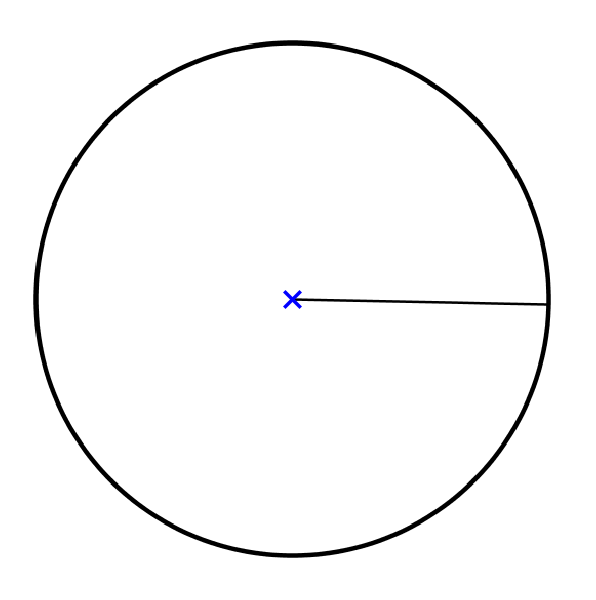
\includegraphics[scale=0.9]{diagramme.eps} \hspace*{0.5cm} 
\includegraphics[scale=0.7]{legende.eps} \\
 \hspace*{10.5cm} \textit{Colorier/hachurer les secteurs et la légende}\\
 
 
 \q "Plus de 50 \% des parisiens interrogés se déplace à pied." Cette affirmation est-elle vraie ou fausse ? \textit{Justifier votre réponse à l'aide d'un calcul.}\\
\reponse[3]\\

\end{document}
